\documentclass{beamer}
\usepackage{lmodern}% http://ctan.org/pkg/lm
\usepackage{amsmath}
\usepackage{color}
\usepackage{tikz}
\usetikzlibrary{fit,arrows,positioning}
\setbeamercolor{bgcolor}{fg=black,bg=white}

\begin{document}
\title{A Contribution to Rating and Recommendation Systems: Concepts, Development and Evaluation}   
\author{Oliver Diestel} 
\date{\today} 

\frame{\titlepage} 

%\frame{\frametitle{Inhaltsverzeichnis}\tableofcontents} 

\section{Overview} 
\frame{\frametitle{Current Situation (Just an assumption)}
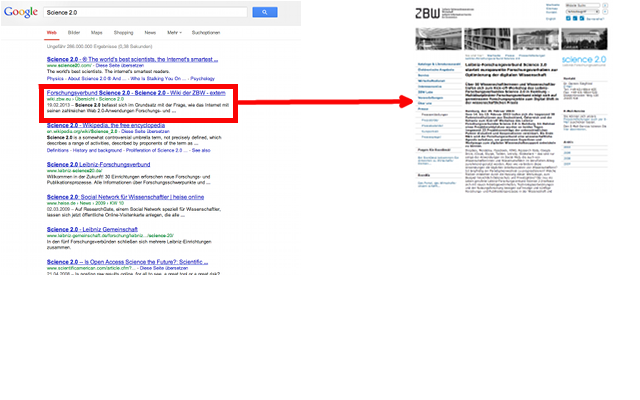
\includegraphics[width=320px, height=200px]{image/google_zbw.png} \\
User visits the zbw.eu website and searchs for the information that he would like to have.
Leaves the website.
}
\frame{\frametitle{Possible Situation}
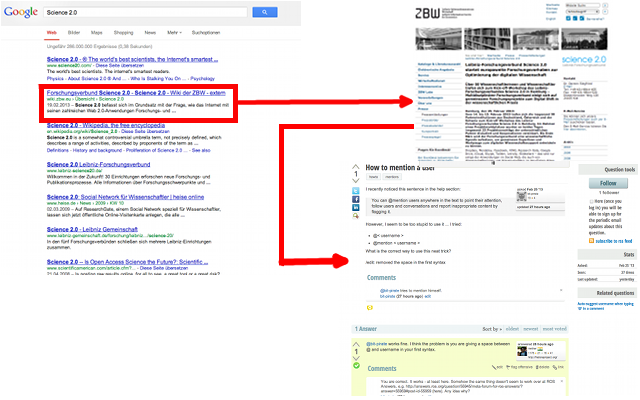
\includegraphics[width=320px, height=200px]{image/google_zbw_askbot.png} \\
User visits the website, sees an interesting question from another user, reads the question and the answer, hopefully asks more questions.
Goal: Increase the user interaction on the website.
%User visits the zbw.eu website searchs for the information that he would like to have,
%his attention will be drawn to a question from another user that fits the subject and the interest from the user.
%The user visits the site of the question gets a deeper understanding of the subject and asks more questions out of curiosity.


}
\frame{\frametitle{Q/A System} 
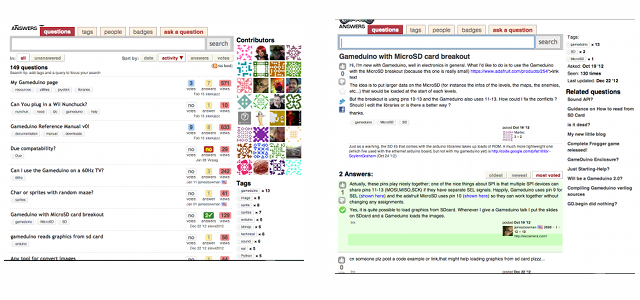
\includegraphics[width=300px]{image/askbot3.png} \\
%Picture of Website / QA with ratings information

%Explanation Question Answer System. (Askbot.com)

General Idea: Use a Question/Answer System to make the information retrieval process public.
Use these public questions and answers to increase the user interaction on the website.

%My part is to bring user relevant information that fits the current subject onto a website.
}
\frame{\frametitle{Beginning}
What do we have at the beginning?\\
Website, Users and Questions\\

%After every new concept answer the question what do we have now
}

\section{Rating}
\frame{\frametitle{Rating}
\begin{itemize}
\item click 
\item active time on page 
\item individual click actions
\end{itemize}

%If a user stays shorter or longer on a page than the average user -  
%it is a high or low rating.\\
%We rate QA pages and webpages, however we only recommend qa pages.
% rating from 1 to 5. 1 if the user bounced, 2 if he stayed a short time 3 average time 4 long time 5 individual action for example he wrote an answer upvoting etc
\pause
What do we have now?\\
Questions, users and the information, which user likes which question 
}

\section{Tagging}
\frame{\frametitle{Tagging}
Find words that describe the question.
\pause
\begin{itemize}
\item STW Thesaurus for Economics %, tripple store
  \pause
\item Stemming: Compute the stem of a word.\\ %(included in 4-Store)
  \pause
  Example rules \\
  "ies" $\rightarrow$ "y" und "s" $\rightarrow$ "" \\
  Examples\\
  "libraries" $\rightarrow$ "library" and "Wikis" $\rightarrow$ "Wiki" 
\pause
\item Computing Levenshtein distance: Calculate the distance between two words.\\
  Example:\\
  Libraries, Librar\textcolor{red}{y}\\
  Distance: 3
\end{itemize}
% \begin{block}{Principle}
% Every question will be tagged with a preferred label from the ZBW Thesaurus.\\
% For every word in the question find the root of the word and match it against the thesaurus.\\
% If we find a matching preferred label, Done. \\
% If we find a matching synonym take the preferd label as tag, Done.
% \end{block}

\pause
What do we have now?\\
Information about which user likes which question and one or more preferred label(s) that describe(s) the subject of the question

}

\section{Recommendation}

%display this enumeration as a black box
\tikzstyle{a} = [rectangle, draw, fill=black, node distance=3cm, text width=5em, text centered, rounded corners, minimum height=4em, thick]
\tikzstyle{b} = [rectangle, draw, fill=white, node distance=3cm, text width=11em, text centered, rounded corners, minimum height=4em, thick]
\tikzstyle{c} = [rectangle, draw, fill=white, node distance=3cm, text width=8em, text centered, rounded corners, minimum height=4em, thick]
\tikzstyle{l} = [draw, -latex',thick]
\frame{\frametitle{Input/Output}
  \begin{columns}
    \begin{column}{6cm}
      \begin{itemize}
        \item Item: id, name, one or more preferred label(s)
        \item User: id, name
      \end{itemize}

%     Question: How does this black box work?
%     Three part recommendation. Pipeline architecture
%     \begin{itemize}
%       \item Calculate similarity between items
%       \item Add similar ratings to a user/rating vector.
%       \item Calculate singular value decomposition
%       \item Find similar users 
%     \end{itemize}
    \end{column}

    \begin{column}{5cm}
      \begin{tikzpicture}[auto]
        \node [b] (input) {$\langle$user\_id, item\_id, rating$\rangle$\\ List(preferred labels)\\ \#recommendations};
        \node [a, below of=input] (blackbox) {\textcolor{white}{blackbox}};
        \node [c, below of=blackbox] (output) {List((item, rating))};
        \path [l] (input) -- (blackbox);
        \path [l] (blackbox) -- (output);
      \end{tikzpicture}
      %Sorted list of Items with approx. user rating that correspond with the pref. input label
    \end{column}
  \end{columns}

}


\frame{\frametitle{Item-Based Algorithm}
%To find similar users we need as much user/item ratings as possible so we would like to guess as much ratings as possible.
  \begin{tabular}{c c c c c c}
   &Item1 & Item2 & Item3 & Item4 & Item5 \\ 
  User1 & 5 & 3 & 4 & 4 & ?\\  
  User2 & 3 & 1 & 2 & 3 & 3\\ 
  User3 & 4 & 3 & 4 & 3 & 5\\ 
  User4 & 3 & 3 & 1 & 5 & 4\\ 
  User5 & 1 & 5 & 5 & 2 & 1\\ 
  \end{tabular}

% \begin{tabular}{c c c c c c}
%  &User1 & User2 & User3 & User4 & User5 \\ 
% Item1 & 5 & 3 & 4 & 3 & 1\\  
% Item2 & 3 & 1 & 3 & 3 & 5\\ 
% Item3 & 4 & 2 & 4 & 1 & 5\\ 
% Item4 & 4 & 3 & 3 & 5 & 2\\ 
% Item5 & ? & 3 & 5 & 4 & 1\\ 
% \end{tabular}


%Find items that have similar ratings.
%Calculate the similarity values for every item.
\pause
\begin{block}{Cosinus Similarity}
  %def calc(a: List[Int], b: List[Int]): Double = {a.zip(b).map((a: (Int, Int)) => a._1*a._2).sum / (Math.sqrt(a.map(Math.pow(_, 2)).sum) * Math.sqrt(b.map(Math.pow(_,2)).sum)).toDouble}
\begin{math}
  sim(\overrightarrow{a}, \overrightarrow{b}) = {\overrightarrow{a} \cdot \overrightarrow{b} \over |\overrightarrow{a}|\cdot|\overrightarrow{b}|}
\end{math}
\end{block}
\begin{block}{Example}
    sim(Item5,Item1) 
  \begin{math}
    = {{3\cdot3 + 5\cdot4 + 4\cdot3 + 1\cdot1} \over {\sqrt{3^2 + 5^2 + 4^2 + 1^2} \cdot \sqrt{3^2 + 4^2 + 3^2 + 1^2}}} = 0.99
  \end{math}
\end{block}

% Take the differences of the average rating behaviour of the user into account.

% \begin{block}{Advanced Cosinus Similarity}
% \begin{math}
%   sim(a, b) = {\sum_{u \in U}(r_{u, a} - \overline{r_u})(r_{u,b} - \overline{r_u}) \over \sqrt{\sum_{u \in U}(r_{u,a} - \overline{r_u})^2} \sqrt{\sum_{u \in U}(r_{u,b} - \overline{r_u})^2 }}
% \end{math}
% \end{block}
}
\frame{\frametitle{Predictions}
%Calculate predictions for similar items.\\
  \begin{block}{Prediction}
    User u, Item p, Rating r_{u, p}\\
    \begin{math}
      pred(u, p) = {\sum_{i \in ratedItems(u)} sim(i, p) \cdot r_{u, i} \over \sum_{i \in ratedItems(u)} sim(i, p)}
    \end{math}
  \end{block}

  \pause

  \begin{block}{Example}
    sim(Item5, Item1) = 0.99\\
    sim(Item5, Item2) = 0.74\\
    sim(Item5, Item3) = 0.72\\
    sim(Item5, Item4) = 0.94\\
    \begin{math}
      pred(User1, I5) = {{0.99 \cdot 5 + 0.74 \cdot 3 + 0.72 \cdot 4 + 0.94 \cdot 4} \over {0.99 + 0.74 + 0.72 + 0.94}} = 4.07
    \end{math}
  \end{block}

%Fill recommendation vector of each user with similar item ratings 
}
\frame{\frametitle{What do we have now?}
  Matrix with less empty fields than before.\\
  \begin{tabular}{c c c c c c}
     &Item1 & Item2 & Item3 & Item4 & Item5 \\ 
     User1 & 5 & 3 & 4 & 4 & \textcolor{red}{4}\\  
    User2 & 3 & 1 & 2 & 3 & 3\\ 
    User3 & 4 & 3 & 4 & 3 & 5\\ 
    User4 & 3 & 3 & 1 & 5 & 4\\ 
    User5 & 1 & 5 & 5 & 2 & 1\\ 
  \end{tabular}

% \begin{tabular}{c c c c c c}
%  &User1 & User2 & User3 & User4 & User5 \\ 
% Item1 & 5 & 3 & 4 & 3 & 1\\  
% Item2 & 3 & 1 & 3 & 3 & 5\\ 
% Item3 & 4 & 2 & 4 & 1 & 5\\ 
% Item4 & 4 & 3 & 3 & 5 & 2\\ 
% Item5 & \textcolor{red}{4} & 3 & 5 & 4 & 1\\ 
% \end{tabular}



}
\frame{\frametitle{Singular Value Decomposition}

  %Now we would like to find similar users with our matrix
  \begin{center}
    ~
    \begin{beamercolorbox}[rounded=true, center, shadow=false,wd=6cm]{bgcolor}
      \begin{math}
        M = \begin{pmatrix} m_{11} & m_{12} & m_{13} \\ m_{21} & m_{22} & m_{23} \\ m_{31} & m_{32} & m_{33}\end{pmatrix}
      \end{math}
    \end{beamercolorbox}
    ~
  \end{center}

  Create a SVD with the matrix 
  \begin{math}
    M = U \cdot \Sigma \cdot V^t
  \end{math}
   %explanations for u sigma and v

  \begin{block}{}
    \begin{columns}
      \begin{column}{4cm}
        \pause
        \begin{math}
          \begin{pmatrix} u_{11} & u_{12} & u_{13} \\ u_{21} & u_{22} & u_{23} \\ u_{31} & u_{32} & u_{33} \end{pmatrix}
        \end{math}
        \begin{block}{}
          %U dimension m x m\\ orthogonal matrix\\ 
          corresponds to the row vectors of matrix m
          \hfill
        \end{block}
      \end{column}
      \begin{column}{4cm}
        \pause
        \begin{math}
          \begin{pmatrix} \sigma_{11} & 0 & 0 \\ 0 & \sigma_{22} & 0 \\ 0 & 0 & \sigma_{33} \end{pmatrix}
        \end{math}
        \begin{block}{}
          %$\Sigma$ dimension m x n\\ 
          diagonal matrix\\ with $\sigma_{ii} > 0$ and $\sigma_{ii} \geq \sigma_{i+1 i+1}$
        \end{block}
      \end{column}
      \begin{column}{4cm}
        \pause
        \begin{math}
          \begin{pmatrix} v_{11} & v_{12} & v_{13} \\ v_{21} & v_{22} & v_{23} \\ v_{31} & v_{32} & v_{33} \end{pmatrix}
        \end{math}
        \begin{block}{}
          %V dimension n x n\\ orthogonal matrix\\ 
          corresponds to the column vectors of matrix m
          \hfill
        \end{block}
      \end{column}
    \end{columns}
  \end{block}




  %Calculate cosinus similarity between users

  %Now we have a two dimensional matrix, so we can calculate the cosinus similarity between our users.
  %Display a graph with the users, show which users are similar display the original matrix next to the graph to validate the result.
}

\frame{\frametitle{Low Rank Approximation of M}
\footnotesize
    \begin{columns}
      \begin{column}{3cm}
        \begin{math}
          \begin{pmatrix} m_{11} & m_{12} & m_{13}\\ m_{21} & m_{22} & m_{23} \\ m_{31} & m_{32} & m_{33} \end{pmatrix} =
        \end{math}
      \end{column}
      \begin{column}{3cm}
        \begin{math}
          \begin{pmatrix} u_{11} & u_{12} & u_{13} \\ u_{21} & u_{22} & u_{23} \\ u_{31} & u_{32} & u_{33} \end{pmatrix} \cdot
        \end{math}
      \end{column}
      \begin{column}{3cm}
        \begin{math}
          \begin{pmatrix} \sigma_{11} & 0 & 0 \\ 0 & \sigma_{22} & 0 \\ 0 & 0 & \sigma_{33} \end{pmatrix} \cdot
        \end{math}
      \end{column}
      \begin{column}{3cm}
        \begin{math}
          \begin{pmatrix} v_{11} & v_{21} & v_{31} \\ v_{12} & v_{22} & v_{32} \\ v_{13} & v_{23} & v_{33} \end{pmatrix}
        \end{math}
      \end{column}
    \end{columns}
  \normalsize

  \begin{block}{}
    \begin{itemize}
    \item Derive from $\Sigma$ the matrix $\Sigma_k$ (with k new rank of M) formed by replacing $\sigma_{ii}$ with $i > k$ by zeros.
      \item Compute and output $M_k = U \cdot \Sigma_k \cdot V^T$  as the rank-k approximation to M.
    \end{itemize}
  \end{block}
  

}

\frame{\frametitle{Low Rank Approximation of M}
\footnotesize
    \begin{columns}
      \begin{column}{3cm}
        \begin{math}
          M_2 =
        \end{math}
      \end{column}
      \begin{column}{3cm}
        \begin{math}
          \begin{pmatrix} u_{11} & u_{12} & u_{13} \\ u_{21} & u_{22} & u_{23} \\ u_{31} & u_{32} & u_{33} \end{pmatrix} \cdot
        \end{math}
      \end{column}
      \begin{column}{3cm}
        \begin{math}
          \begin{pmatrix} \sigma_{11} & 0 & 0 \\ 0 & \sigma_{22} & 0 \\ 0 & 0 & 0 \end{pmatrix} \cdot
        \end{math}
      \end{column}
      \begin{column}{3cm}
        \begin{math}
          \begin{pmatrix} v_{11} & v_{21} & v_{31} \\ v_{12} & v_{22} & v_{32} \\ v_{13} & v_{23} & v_{33} \end{pmatrix}
        \end{math}
      \end{column}
    \end{columns}
  \normalsize

  \begin{block}{}
    \begin{itemize}
    \item Derive from $\Sigma$ the matrix $\Sigma_k$ (with k new rank of M) formed by replacing $\sigma_{ii}$ with $i > k$ by zeros.
      \item Compute and output $M_k = U \cdot \Sigma_k \cdot V^T$  as the rank-k approximation to M.
    \end{itemize}
  \end{block}
  

}

\frame{\frametitle{Low Rank Approximation of M}
\footnotesize
    \begin{columns}
      \begin{column}{3cm}
        \begin{math}
          M_2 =
        \end{math}
      \end{column}
      \begin{column}{3cm}
        \begin{math}
          \begin{pmatrix} \textcolor{red}{u_{11}} & \textcolor{green}{u_{12}} & \textcolor{blue}{u_{13}} \\ u_{21} & u_{22} & u_{23} \\ u_{31} & u_{32} & u_{33} \end{pmatrix} \cdot
        \end{math}
      \end{column}
      \begin{column}{3cm}
        \begin{math}
          \begin{pmatrix} \textcolor{red}{\sigma_{11}} & 0 & 0 \\ \textcolor{green}{0} & \sigma_{22} & 0 \\ \textcolor{blue}{0} & 0 & 0 \end{pmatrix} \cdot
        \end{math}
      \end{column}
      \begin{column}{3cm}
        \begin{math}
          \begin{pmatrix} v_{11} & v_{21} & v_{31} \\ v_{12} & v_{22} & v_{32} \\ v_{13} & v_{23} & v_{33} \end{pmatrix}
        \end{math}
      \end{column}
    \end{columns}

    \begin{block}{}
      \begin{columns}
        \begin{column}{3cm}
          \begin{math}
            M_2 =
          \end{math}
        \end{column}
        \begin{column}{6cm}
          \hfill
          \begin{math}
            \begin{pmatrix} u_{11} \cdot \sigma_{11} & u_{12} \cdot \sigma_{22} & u_{13} \cdot 0  \\ u_{21} \cdot \sigma_{11} & u_{22} \cdot \sigma_{22} & u_{23} \cdot 0 \\ u_{31} \cdot \sigma_{11} & u_{32} \cdot \sigma_{22} & u_{33} \cdot 0 \end{pmatrix} \cdot
          \end{math}
          \hfill\hfill
        \end{column}
        \begin{column}{3cm}
          \begin{math}
            \begin{pmatrix} v_{11} & v_{21} & v_{31} \\ v_{12} & v_{22} & v_{32} \\ v_{13} & v_{23} & v_{33} \end{pmatrix}
          \end{math}
        \end{column}
      \end{columns}
    \end{block}

  \normalsize

}

\frame{\frametitle{Low Rank Approximation of M}
\footnotesize
    \begin{columns}
      \begin{column}{3cm}
        \begin{math}
          M_2 =
        \end{math}
      \end{column}
      \begin{column}{3cm}
        \begin{math}
          \begin{pmatrix} \textcolor{red}{u_{11}} & \textcolor{green}{u_{12}} & \not{\textcolor{blue}{u_{13}}} \\ u_{21} & u_{22} & \not{u_{23}} \\ u_{31} & u_{32} & \not{u_{33}} \end{pmatrix} \cdot
        \end{math}
      \end{column}
      \begin{column}{3cm}
        \begin{math}
          \begin{pmatrix} \textcolor{red}{\sigma_{11}} & 0 & 0 \\ \textcolor{green}{0} & \sigma_{22} & 0 \\ \textcolor{blue}{0} & 0 & 0 \end{pmatrix} \cdot
        \end{math}
      \end{column}
      \begin{column}{3cm}
        \begin{math}
          \begin{pmatrix} v_{11} & v_{21} & v_{31} \\ v_{12} & v_{22} & v_{32} \\ v_{13} & v_{23} & v_{33} \end{pmatrix}
        \end{math}
      \end{column}
    \end{columns}

    \begin{block}{}
      \begin{columns}
        \begin{column}{3cm}
          \begin{math}
            M_2 =
          \end{math}
        \end{column}
        \begin{column}{6cm}
          \hfill
          \begin{math}
            \begin{pmatrix} u_{11} \cdot \sigma_{11} & u_{12} \cdot \sigma_{22} & u_{13} \cdot 0  \\ u_{21} \cdot \sigma_{11} & u_{22} \cdot \sigma_{22} & u_{23} \cdot 0 \\ u_{31} \cdot \sigma_{11} & u_{32} \cdot \sigma_{22} & u_{33} \cdot 0 \end{pmatrix} \cdot
          \end{math}
          \hfill\hfill
        \end{column}
        \begin{column}{3cm}
          \begin{math}
            \begin{pmatrix} v_{11} & v_{21} & v_{31} \\ v_{12} & v_{22} & v_{32} \\ v_{13} & v_{23} & v_{33} \end{pmatrix}
          \end{math}
        \end{column}
      \end{columns}
    \end{block}

  \normalsize

}




\frame{\frametitle{Example SVD}
\tiny
\begin{math}
  \begin{tabular}{c c c c c c}
     &Item1 & Item2 & Item3 & Item4 & Item5 \\ 
     User1 & 5 & 3 & 4 & 4 & 4\\  
    User2 & 3 & 1 & 2 & 3 & 3\\ 
    User3 & 4 & 3 & 4 & 3 & 5\\ 
    User4 & 3 & 3 & 1 & 5 & 4\\ 
    User5 & 1 & 5 & 5 & 2 & 1\\ 
  \end{tabular} = 
  \pause

  \begin{pmatrix}
    0.544178 & 0.0875457 & 0.303701 & -0.598262 & -0.496039 \\ 0.330582 & 0.270665 & 0.155794 & -0.281254 & 0.845033 \\ 0.517601 & 0.04377 & 0.429477 & 0.737011 & -0.0503875 \\ 0.438285 & 0.373564 & -0.800903 & 0.129864 & -0.100232 \\ 0.366854 & -0.881822 & -0.239996 & -0.0541261 & 0.165165
  \end{pmatrix} \cdot \\
  \begin{pmatrix}
    16.499 & 0 & 0 & 0 & 0 \\ 0 & 4.93905 & 0 & 0 & 0 \\ 0 & 0 & 2.58239 & 0 & 0 \\ 0 & 0 & 0 & 1.20841 & 0 \\ 0 & 0 & 0 & 0 & 0.511218
  \end{pmatrix} \cdot \\
  \begin{pmatrix} 
    0.452438 & 0.336841 & 0.410894 & -0.456436 & -0.55197 \\ 0.403968 & -0.531238 & -0.483027 & 0.210155 & -0.526419 \\ 0.43523 & -0.601119 & 0.481498 & -0.122706 & 0.449817 \\ 0.463447 & 0.282982 & -0.586236 & -0.401113 & 0.447854 \\ 0.477391 & 0.403612 & 0.149459 &  0.756011 &  0.12371
  \end{pmatrix}^T
\end{math}
\normalsize
}

\frame{\frametitle{Diagram of SVD}
\footnotesize
\begin{columns}
  \begin{column}{7cm}
\begin{math}
  \begin{tabular}{c c c c c c}
     &Item1 & Item2 & Item3 & Item4 & Item5 \\ 
     User1 & 5 & 3 & 4 & 4 & 4\\  
    User2 & 3 & 1 & 2 & 3 & 3\\ 
    User3 & 4 & 3 & 4 & 3 & 5\\ 
    User4 & 3 & 3 & 1 & 5 & 4\\ 
    User5 & 1 & 5 & 5 & 2 & 1\\ 
  \end{tabular} 

  \begin{block}{}
  \begin{pmatrix}
    0.544178 & 0.0875457  \\ 0.330582 & 0.270665  \\ 0.517601 & 0.04377 \\ 0.438285 & 0.373564  \\ 0.366854 & -0.881822 
  \end{pmatrix} 
\end{block}
\end{math}
\pause
\end{column}
\begin{column}{4cm}
\noindent
\begin{tikzpicture}[scale=3.0]
 \begin{scope}[thin,black,dot/.style={fill=blue,circle,inner sep=0pt,minimum size=3pt}]
   %x-y-Koordinatensystem
%  \draw[-latex] (90:-1) --++(90:2) node[left]{$y$};
%  \draw[-latex] (0:-1) --++(0:2) node[below]{$x$};
   \coordinate (x1) at (0, 0);
   \coordinate (x2) at (1, 0);
   \coordinate (y1) at (0, -1);
   \coordinate (y2) at (0, 1);
   \draw (x1) -- (x2) node[right]{$x$};
   \draw (y1) -- (y2) node[above]{$y$};
   \node [left] at (0,0) {$0.0$};
   \node [left] at (0,-1) {$-1.0$};
   \node [left] at (0,1) {$1.0$};
   \node [below] at (1,0) {$1.0$};


   \coordinate (user1) at (0.544178, 0.0875457); 
   \node[dot] at (user1);
   \node [anchor=west] at (user1) {$User1$};

   \coordinate (user2) at (0.330582, 0.270665); 
   \node[dot] at (user2);
   \node [anchor=west] at (user2) {$User2$};

   \coordinate (user3) at (0.517601, 0.04377); 
   \node[dot] at (user3);
   \node [anchor=north west] at (user3) {$User3$};

   \coordinate (user4) at (0.438285, 0.373564); 
   \node[dot] at (user4);
   \node [anchor=west] at (user4) {$User4$};

   \coordinate (user5) at (0.366854, -0.881822); 
   \node[dot] at (user5);
   \node [anchor=west] at (user5) {$User5$};

   

   
 \end{scope}
\end{tikzpicture}
\end{column}
\end{columns}

\pause
Recommendations for User 
\begin{itemize}
  \item Take the k most similar users SU
  \item Take the top k unknown items (with the right context) from each user $\in$ SU
  \item Use cosinus similarity for rating weighting
\end{itemize}
\normalsize
}

\frame{\frametitle{Is this a good approach?}
\begin{itemize}
  \item We could have calculated the SVD directly out of the original matrix. Would we get a similar result?
    \pause
  \item Is it better if we use the V matrix from the SVD to calculate the item similarity and update the SVD afterwards?
    \pause
  \item Is it better if we just recommend similar items from the items the user already likes?
    \pause
  \item Should we use cosinus similarity between the users in the first place.
\end{itemize}
}

\frame{\frametitle{Evaluation}
  The test data: I use real data from the zbw econdesk. However, we do not have real user ratings for this data.
  \begin{itemize}
    \item Every data gets a random quality value from 1 (rather negative rating) to 5 (rather positive rating). %if a user would rather rate it positive or negative.
    \item Furthermore, I generate 1000 test users. These users will have a rating preferation. So a user might be a person that rates an item more positive or more negative.
    \item I will try to evaluate the algorithms with this test data. I might use a movie db as well for this.
  \end{itemize}

}

\section{Display Information}
% \frame{\frametitle{Find Questions}
% Find questions that are hightly rated by similar users that match the current topic
% }

% \frame{\frametitle{Display Questions}
% Add a tag and  a div-placeholder on every webpage. Display top questions for the current user on the webpage.

% }

\section{Software Architecture}

\frame{\frametitle{Software Architecture}
Scala: Finagle twitter framework\\
Every part of the software is a service.  \\
The tagger, the rating algorithm and the recommendation algorithms can be used as an individual software. \\

}

\section{Timtable}
\frame{\frametitle{Timetable}
Start: 18.12.2012\\
End: 18.06.2013\\

1st month(18.01): Theory\\
2nd month(18.02): Theory + Technology\\ 
3rd month(18.03): Implementation\\
4th month(18.04): Implementation + First writings\\
5th month(18.05): Final thesis\\
Personal Goal\\
Technology implemented: 31.03.2013 \\
Diplom Thesis ready: 01.05.2013
}

% \section{Abschnitt Nr. 2} 
% \subsection{Listen I}
% \frame{\frametitle{Aufz\"ahlung}
% \begin{itemize}
% \item Einf\"uhrungskurs in \LaTeX  
% \item Kurs 2  
% \item Seminararbeiten und Pr\"asentationen mit \LaTeX 
% \item Die Beamerclass 
% \end{itemize} 
% }

% \frame{\frametitle{Aufz\"ahlung mit Pausen}
% \begin{itemize}
% \item  Einf\"uhrungskurs in \LaTeX \pause 
% \item  Kurs 2 \pause 
% \item  Seminararbeiten und Pr\"asentationen mit \LaTeX \pause 
% \item  Die Beamerclass
% \end{itemize} 
% }

% \subsection{Listen II}
% \frame{\frametitle{Numerierte Liste}
% \begin{enumerate}
% \item  Einf\"uhrungskurs in \LaTeX 
% \item  Kurs 2
% \item  Seminararbeiten und Pr\"asentationen mit \LaTeX 
% \item  Die Beamerclass
% \end{enumerate}
% }
% \frame{\frametitle{Numerierte Liste mit Pausen}
% \begin{enumerate}
% \item  Einf\"uhrungskurs in \LaTeX \pause 
% \item  Kurs 2 \pause 
% \item  Seminararbeiten und Pr\"asentationen mit \LaTeX \pause 
% \item  Die Beamerclass
% \end{enumerate}
% }

% \section{Abschnitt Nr.3} 
% \subsection{Tabellen}
% \frame{\frametitle{Tabellen}
% \begin{tabular}{|c|c|c|}
% \hline
% \textbf{Zeitpunkt} & \textbf{Kursleiter} & \textbf{Titel} \\
% \hline
% WS 04/05 & Sascha Frank &  Erste Schritte mit \LaTeX  \\
% \hline
% SS 05 & Sascha Frank & \LaTeX \ Kursreihe \\
% \hline
% \end{tabular}}


% \frame{\frametitle{Tabellen mit Pause}
% \begin{tabular}{c c c}
% A & B & C \\ 
% \pause 
% 1 & 2 & 3 \\  
% \pause 
% A & B & C \\ 
% \end{tabular} }


% \section{Abschnitt Nr. 4}
% \subsection{Bl\"ocke}
% \frame{\frametitle{Bl\"ocke}

% \begin{block}{Blocktitel}
% Blocktext 
% \end{block}

% \begin{exampleblock}{Blocktitel}
% Blocktext 
% \end{exampleblock}


% \begin{alertblock}{Blocktitel}
% Blocktext 
% \end{alertblock}
% }
\end{document}

